
The following script shows how to analyse root system length versus time. 

\lstinputlisting[language=Python, caption=Organ development over time]{examples/topics_development.py}

\begin{itemize}
\item[9-14] Sets up the simulation.

\item[16-18] Defines the simulation time, time step, and the resulting number of simulate(dt) calls. 

\item[21] First we state which scalar type we want to analyse ('volume', 'surface', or 'one' would also make sense). 

\item[22] Pre-definition of the numpy arrays storing the lengths over time. 

\item[23-30] The simulation loop executes the simulation for a single time step L24. L25 calculates the type of each root (the organ subType), L26 the length (or any other parameter) of the root. L27-L30 calculates the total root length at the current time step for all roots, and for specific root types. The method rs.getParameter collects this data from the RootSystem organs. It is possible to access all root random parameters and resulting realisations using rs.getParameter. In C++ the class functions are defined in Root::getParameter, Organ::getParameter. 

\item[32-38] Creates Figure \ref{fig:length}.

\end{itemize}



Next we show two options how to retrieve root tip and root base positions from a simulation:

\lstinputlisting[language=Python, caption=Organ tips and organ bases over time]{examples/topics_development2.py}

\begin{itemize}

\item[14,15] Reset the simulation and simulate for only 7 days (otherwise there are so many root tips).

\item[17-18] Outputs the number of nodes and segments to get an idea how big the resulting root system is. 
Note that number of segments equals the number of nodes minus the number of base roots that will emerge. 
Base roots are tap roots, basal roots and shootborne roots.

\item[20-26] The first approach retrieves all roots as polylines L21. 
Root tips are the last nodes of the polylines L26, root bases the first nodes L25. Roots that have not started to grow have only 1 node, and are not retrieved by getPolylines().

\item[28-31] Second approach: L29 rs.getNodes() returns all nodes of the root system as a list of nodes, i.e. Vector3d objects. Each Vector3d object can be converted into a numpy array automatically, but is necessary to do that for each element of the list. The methods L30, L31 return the indices of the tips and bases. 

\item[33-41] Creates Figure \ref{fig:scatter} using the second approach.

\item[44,45] Verifies that both approaches yield the same result.

\end{itemize}

\begin{figure}
\begin{subfigure}[c]{0.5\textwidth}
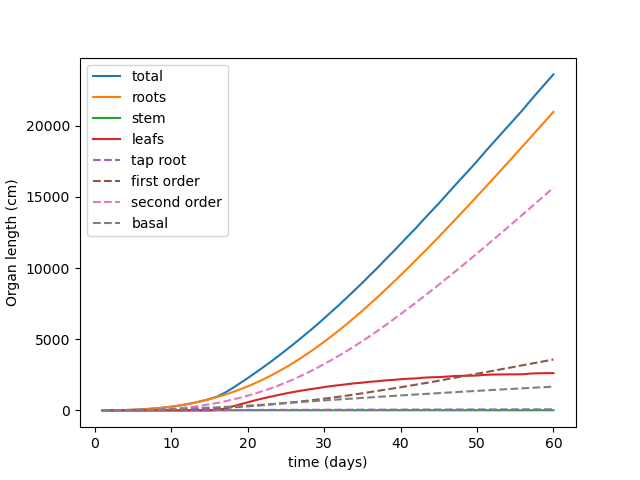
\includegraphics[width=0.99\textwidth]{examples/results/topics_development.png}
\subcaption{Total organ lengths versus time} \label{fig:topics_development}
\end{subfigure}
\begin{subfigure}[c]{0.5\textwidth}
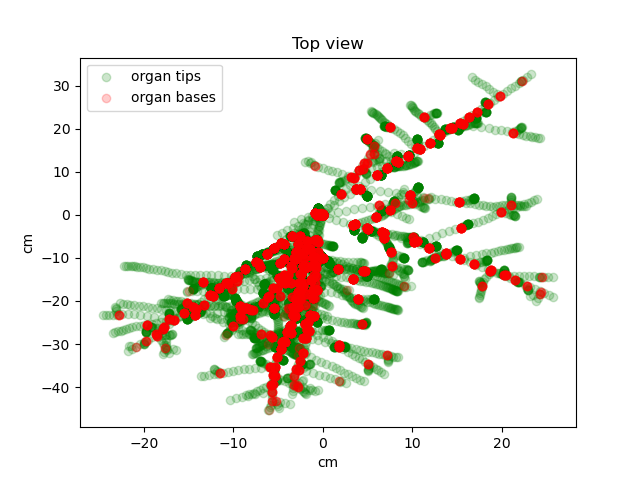
\includegraphics[width=0.99\textwidth]{examples/results/topics_development2.png}
\subcaption{Top view of the organ tip and bases} \label{fig:topics_development2}
\end{subfigure}
\caption{Plant development over time} 
\end{figure}


